%% LaTeX-Beamer template for KIT design
%% by Erik Burger, Christian Hammer
%% title picture by Klaus Krogmann
%%
%% version 2.1
%%
%% mostly compatible to KIT corporate design v2.0
%% http://intranet.kit.edu/gestaltungsrichtlinien.php
%%
%% Problems, bugs and comments to
%% burger@kit.edu

\documentclass[18pt]{beamer}
\usepackage[utf8x]{inputenc}
\usepackage{units}
\usepackage{booktabs}


%% SLIDE FORMAT

% use 'beamerthemekit' for standard 4:3 ratio
% for widescreen slides (16:9), use 'beamerthemekitwide'

%\usepackage{templates/beamerthemekit}
 \usepackage{templates/beamerthemekitwide}

%% TITLE PICTURE

% if a custom picture is to be used on the title page, copy it into the 'logos'
% directory, in the line below, replace 'mypicture' with the 
% filename (without extension) and uncomment the following line
% (picture proportions: 63 : 20 for standard, 169 : 40 for wide
% *.eps format if you use latex+dvips+ps2pdf, 
% *.jpg/*.png/*.pdf if you use pdflatex)

%\titleimage{mypicture}

%% TITLE LOGO

% for a custom logo on the front page, copy your file into the 'logos'
% directory, insert the filename in the line below and uncomment it

%\titlelogo{mylogo}
\titlelogo{}

% (*.eps format if you use latex+dvips+ps2pdf,
% *.jpg/*.png/*.pdf if you use pdflatex)

%% TikZ INTEGRATION

% use these packages for PCM symbols and UML classes
% \usepackage{templates/tikzkit}
% \usepackage{templates/tikzuml}

% the presentation starts here

\title[GBI Tutorium]{GBI Tutorium Nr. }
\subtitle{Foliensatz 01}
\date{23. Oktober 2012}
\author{Vincent Hahn -- vincent.hahn@student.kit.edu}

\institute{Institut für theoretische Informatik}

% Bibliography

%\usepackage[citestyle=authoryear,bibstyle=numeric,hyperref,backend=biber]{biblatex}
%\addbibresource{templates/example.bib}
%\bibhang1em

\begin{document}

% change the following line to "ngerman" for German style date and logos, english: english
\selectlanguage{ngerman}

%title page
\begin{frame}
\titlepage
\end{frame}

%table of contents
\begin{frame}{Outline/Gliederung}
\tableofcontents
\end{frame}

\section{Allgemeines}
\begin{frame}{Kontaktmöglichkeiten}
\begin{itemize}
    \item Mail: \href{mailto:vincent.hahn@student.kit.edu}{vincent.hahn@student.kit.edu}
\pause
    \item Web: \url{http://www.stud.uni-karlsruhe.de/~uddgw/}
\end{itemize}
\end{frame}

\begin{frame}{Termine}
    \begin{itemize}
    \item Übungsblattabgabe:
    \pause
    \item Übung: 
    \item Vorlesung: 
    \pause
    \item Klausurtermin: gewöhnlich Anfang März des kommenden Jahres
    \end{itemize}
\end{frame}

\begin{frame}{Übungsblatter}
    Die Übungsbläter müssen\dots
    \begin{itemize}
        \item handbeschrieben sein,
        \item mit Deckblatt abgeben werden und
        \item selbst bearbeiten sein.
    \end{itemize}
    Für den Übungsschein reichen $\unit[50]{\%}$ der Punkte der Blätter.
\end{frame}

\begin{frame}{Weitere Links}
    \begin{block}{Vorlesung}
        \begin{itemize}
            \item Website: \url{http://gbi.ira.uka.de}
            \item Dozentin: \href{mailto:tanja.schultz@kit.edu}{tanja.schultz@kit.edu}
        \end{itemize}
    \end{block}
    \pause
    \begin{block}{Fachschaft}
        \begin{itemize}
            \item Website: \url{http://www.fsmi.uni-karlsruhe.de/}
            \item Forum: \url{http://www.fsmi.uni-karlsruhe.de/forum/}
        \end{itemize}
    \end{block}
\end{frame}



\section{Aussagenlogik}
\begin{frame}{Junktoren}
    \begin{block}{Definition}
        Ein Junktor ist eine logische Verknüpfung zwischen Aussagen innerhalb der Aussagenlogik, also ein logischer Operator.\\
        (Aus Wikipedia)
    \end{block}
    \pause
    \begin{exampleblock}{Beispiele}
    \begin{itemize}
        \item Logisches "`Oder"' $\vee$
        \item Logisches "`Und"' $\wedge$
        \item \dots
    \end{itemize}
    \end{exampleblock}
    \end{frame}

    \begin{frame}{Logisches Und ("`Konjunktion"')}
        \begin{table}
            \caption{Wahrheitswerte für $\wedge$}
            \begin{center}
                \begin{tabular}{ccc}
                    \toprule
                    $A$ & $B$ & $A \wedge B$\\
                    \midrule
                    f & f & f\\
                    f & w & f\\
                    w & f & f\\
                    w & w & w\\
                    \bottomrule
                \end{tabular}
             \end{center}
        \end{table}
    \end{frame}

    \begin{frame}{Logisches Oder "`Disjunktion"'}
        \begin{table}
            \caption{Wahrheitswerte für $\vee$}
            \begin{center}
                \begin{tabular}{ccc}
                    \toprule
                    $A$ & $B$ & $A \vee B$\\
                    \midrule
                    f & f & f\\
                    f & w & w\\
                    w & f & w\\
                    w & w & w\\
                    \bottomrule
                \end{tabular}
             \end{center}
        \end{table}
    \end{frame}

    \begin{frame}{Negation}
        \begin{table}
            \caption{Wahrheitswerte für $\neg$}
            \begin{center}
                \begin{tabular}{ccc}
                    \toprule
                    $A$ & $ \neg A$\\
                    \midrule
                    f & w\\
                    f & f\\
                    \bottomrule
                \end{tabular}
             \end{center}
        \end{table}
    \end{frame}

    \begin{frame}{Subjunktion}
        \begin{table}
            \caption{Wahrheitswerte für $\rightarrow$}
            \begin{center}
                \begin{tabular}{ccc}
                    \toprule
                    $A$ & $B$ & $A \rightarrow B$\\
                    \midrule
                    f & f & w\\
                    f & w & w\\
                    w & f & f\\
                    w & w & w\\
                    \bottomrule
                \end{tabular}
             \end{center}
        \end{table}
        \pause
        \begin{exampleblock}{Alternative Schreibeweise}
            Finde eine Schreibweise, die nur aus $\vee$ und $\neg$ besteht!\\
            \pause
            \invisible<1,2>{$A \rightarrow B \Leftrightarrow \neg A \vee B$}
        \end{exampleblock}
    \end{frame}

    \begin{frame}{Klausuraufgabe}
        \begin{exampleblock}{Sommer 2010, Aufgabe 2\\ 2 von 46 Punkten}
            Zeigen Sie (etwa mit Wahrheitstabellen), dass die Formeln äquivalent sind:
            \begin{align*}
                \left(\left(\left( B \Rightarrow A\right)\vee B\left) \Rightarrow \left(\neg A\right)\right) &\wedge B\\
                \neg A &\wedge B
            \end{align*}
        \end{exampleblock}
    \end{frame}

\section{Eigenschaften von Abbildungen}
    \subsection{Totalität}
        \begin{frame}{Totalität}
            \begin{block}{Definition}
                Eine Relation $R \subseteq A \times B $ heißt linkstotal, wenn es zu jedem Element der Urbildmenge $A$ ein zugehöriges Element der Bildmenge $B$ gibt.\\*


                Die Relation heißt rechtstotal, wenn es zu jedem Element der Bildmenge $B$ ein zugehöriges Element der Urbildmenge $A$ gibt.
            \end{block}
            \pause
            \begin{exampleblock}{Beispiel}
                Welche Eigenschaft hat diese Funktion, wenn $x \in \mathbb{R}$ und $f(x) \in \mathbb{R}$? 
                \begin{align*}
                    f\left(x\right) = x^2
                \end{align*}
                \pause
                \invisible<1-2>{Linkstotal.}
            \end{exampleblock}
        \end{frame}

    \subsection{Eindeutigkeit}
        \begin{frame}{Eindeutigkeit}
            \begin{block}{Definition}
                Eine Relation $R \subseteq A \times B$ heißt linkseindeutig, wenn einem Element der Bildmenge $B$ höchstens ein Element der Urbildmenge $A$ zugeordnet ist.\\


                Eine Relation $R \subseteq A \times B$ heißt rechtseindeutig, wenn einem Element der Urbildmenge $A$ höchstens ein Element der Bildmenge $B$ zugeordnet ist.
            \end{block}
            \pause
            \begin{exampleblock}{Beispiel}
                Welche Eigenschaft hat die Funktion $f(x) = x^2$ (Wertebereiche wie oben)?
                \pause
                \invisible<1-2>{Rechtseindeutig.}
            \end{exampleblock}
        \end{frame}

    \subsection{Funktionen}
    \begin{frame}{Funktionen}
        \begin{block}{Definition}
                Eine Relation $R \subseteq A \times B$ heißt Funktion, wenn sie linkstotal und rechtseindeutig ist.
        \end{block}
        \begin{block}{Eigenschaften einer Funktion}
            \begin{table}
                \centering
                \caption{Eigenschaften von Funktionen. Dabei sei $x \in \mathbb{R}$ und $f\left( x\right)\in \mathbb{R}$ (also keine komplexen Zahlen).}
                \begin{tabular}{llll}
                    \toprule
                    rechtstotal & linkseindeutig & Bezeichnung & Beispiel\\
                    \midrule
                    0 & 0 & - & $f\left( x\right) = x^2$\\
                    0 & 1 & injektiv & $f\left( x \right) = e^x$\\
                    1 & 0 & surjektiv & $f\left( x \right) = x^3 - x$\\
                    1 & 1 & bijektiv & $f\left( x\right) = x$\\
                    \bottomrule
                \end{tabular}
            \end{table}
        \end{block}
    \end{frame}
    \begin{frame}{Graphen}
        \begin{columns}
            \begin{column}{.5\textwidth}
                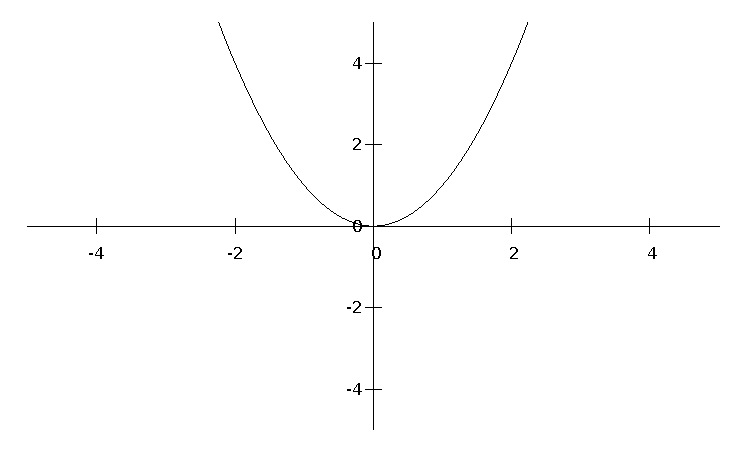
\includegraphics[width=1\textwidth]{graphics/01/01.pdf}
            \end{column}
            \begin{column}{.5\textwidth}
                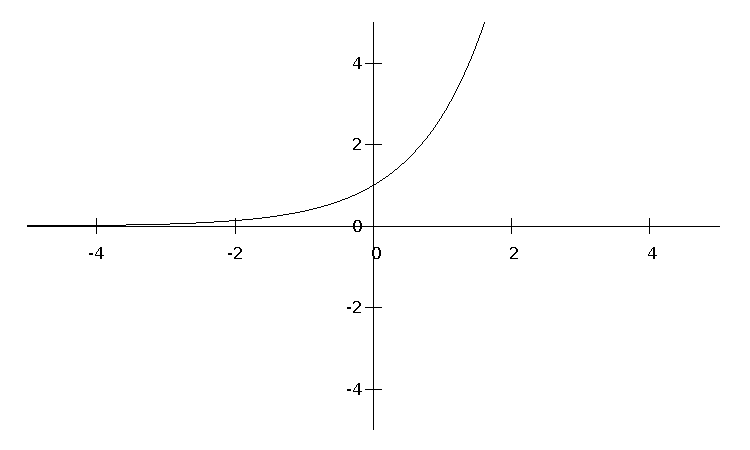
\includegraphics[width=1\textwidth]{graphics/01/02.pdf}
            \end{column}
        \end{columns}
        \begin{columns}
            \begin{column}{.5\textwidth}
                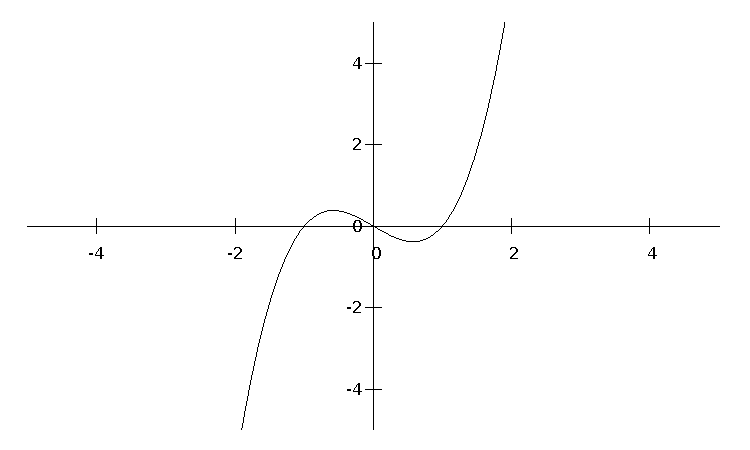
\includegraphics[width=1.\textwidth]{graphics/01/03.pdf}
            \end{column}
            \begin{column}{.5\textwidth}
                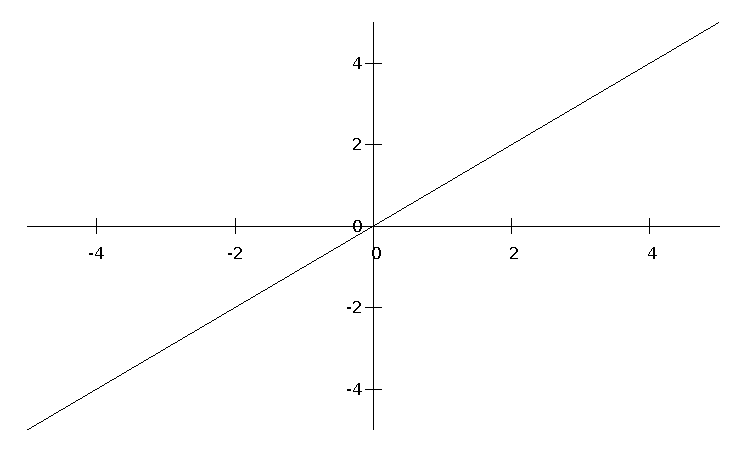
\includegraphics[width=1.\textwidth]{graphics/01/04.pdf}
            \end{column}
        \end{columns}
    \end{frame}
    \begin{frame}{Funktionen}
        \begin{alertblock}{Vorsicht}
            Unbedingt den Definitionsbereich einer Funktion beachten. Die Normalparabel ist im Bereich der komplexen Zahlen surjektiv!
        \end{alertblock}
    \end{frame}
    \begin{frame}{Übungsaufgabe}
        \begin{exampleblock}{Winter 2010/2011, Aufgabe 1.2}
            Es sei $A$ die Menge aller Kinobesucher in einer Vorstellung und $B$ die Menge aller Sitzplätze. Die Abbildung $f$ ordnet den Kinobesuchern die Sitzplätze zu: $ f: A \rightarrow B $
            \begin{itemize}
                \item Was bedeutet es im Kino, wenn $f$ linkstotal, linkseindeutig, rechtstotal, rechtseindeutig ist?
                \item Was wünschen sich die Kinobesucher: Eine injektive, surjektive oder bijektive Abbildung auf die Sitzplätze? Was wünscht sich der Besitzer?
                \item In dieser Teilaufgabe nehmen wir an, 6 Kinobesucher besuchten ein Kino mit 8 Plätzen. Zeichnen Sie eine injektive Abbildung $f$. Wie viele injektive Abbildungen gibt es? 
            \end{itemize}
        \end{exampleblock}
    \end{frame}



\appendix
\beginbackup

%\begin{frame}[allowframebreaks]{References}
%\printbibliography
%\end{frame}

\backupend

\end{document}
